 \section{INTRODU{\c C}ÃO}

O Departamento de Computação da Faculdade de Ciências
da UNESP, campus de Bauru, participa de competições de
futebol de robôs, na modalidade Very Small Size (atualmente
IEEE Very Small), desde 1998, com a realização do 1\textordmasculine
Campeonato Brasileiro de Futebol de Robôs -- CBFR 98. A
pesquisa e o desenvolvimento em futebol de robôs mantém o objetivo de incentivar o uso de
inovações tecnológicas, no campo da robótica, de baixo custo e
com componentes encontrados no mercado nacional. O time de futebol da UNESP
de Bauru é conhecido, desde a primeira edição desta
competição no Brasil, como Carrossel Caipira devido sua
estratégia de jogo. O projeto atual é a sexta versão, de robôs
desenvolvidos para futebol de robôs, com aprimoramentos em
relação ao time de 2017.

No ambiente do futebol de robôs, nesta categoria, os robôs
e a bola são identificados através de uma câmera utilizada
como visão global, posicionada a 2m sobre o campo e alinhada
ao seu centro, que captura imagens da arena. Estas imagens são
processadas digitalmente obtendo as coordenadas dos robôs e da bola.
A partir dessas coordenadas, uma estratégia escolhida e transformada em comandos que são enviados aos
robôs por rádio. Os robôs recebem estes comandos e realizam
as ações correspondentes, modificando a posição dos
elementos presentes no ambiente real, que será capturado
novamente pela câmera. A Fig. \ref{fig:setup_geral} apresenta uma ilustração do
ambiente do futebol de robôs.

% FIGURA
\begin{figure}[!htb]
\centering
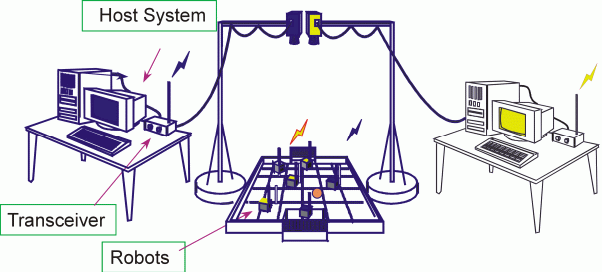
\includegraphics[scale=0.54]{setup_geral1.png}
\caption{Ambiente para futebol de robôs. Fonte:www.mecatronicaatual.com.br/secoes/leitura/950 (2013)}
\label{fig:setup_geral}
\end{figure}
%%%

O futebol robótico abrange diversas áreas do conhecimento.
Na construção do robô são aplicados conceitos de mecânica,
eletrônica e sistemas embarcados. Do ponto de vista do
software, executado no computador pessoal, estão envolvidos
elementos de processamento de imagens, inteligência artificial
e teoria de controle. Essa abrangência faz desta modalidade de
futebol uma ferramenta pedagógica com possíveis aplicações
na graduação.
Esse projeto busca incentivar e facilitar o desenvolvimento
da robótica, para isso o artigo faz uma apresentação das tarefas
realizadas, enfatizando a melhoria aplicada recentemente na arquitetura do software
como um todo e no novo sistema de controle.
